\renewcommand{\thesection}{\Roman{section}}
\section{Methods}

\subsection*{System Overview}

\quad The system consists of the 7-DOF Barrett WAM robot arm and 4-DOF Barrett BH-280 Hand from Barrett Technology, Inc (compare figure \ref{setup}). The robot is equipped with one 6-DOF wrist torque sensor, three 1-DOF finger joint torque sensors, and four 24-DOF tactile pressure sensors, making for a total of 105 independent sensor inputs. Given such rich sensory input, we hoped to obtain feature vectors which exhibit statistically significant differences between different grasp shapes. All the sensors read at 125\,Hz. Most afferent inputs in humans run at less than 60\,Hz, so this rate is sufficient to mimic physiological driven grasping approaches \cite{Howe}.

\begin{figure}[H]
	\centering
	\includegraphics[width=0.46\textwidth]{setup.jpg}	
	\caption{7-DOF Barrett WAM robot arm and 4-DOF Barrett BH-280 Hand from Barrett Technology, Inc.}
	\label{setup}
\end{figure}

\subsection*{Software Architecture}
\label{softarch}
The software for running our experiments on the Barrett WAM and Hand is a menu-based command-line program that makes it easy to record sensor data and test out differently trained neural networks. The hand's home position as well as the initial grasp positions are predefined and can be called individually. On the main operational level, the menu lets the user choose one of 5 different grasp types: \\ \\
\begin{minipage}{0.5\textwidth}
\qquad\quad  \textbf{Top-down Prismatic Precision} 
\begin{figure}[H]
	\centering
	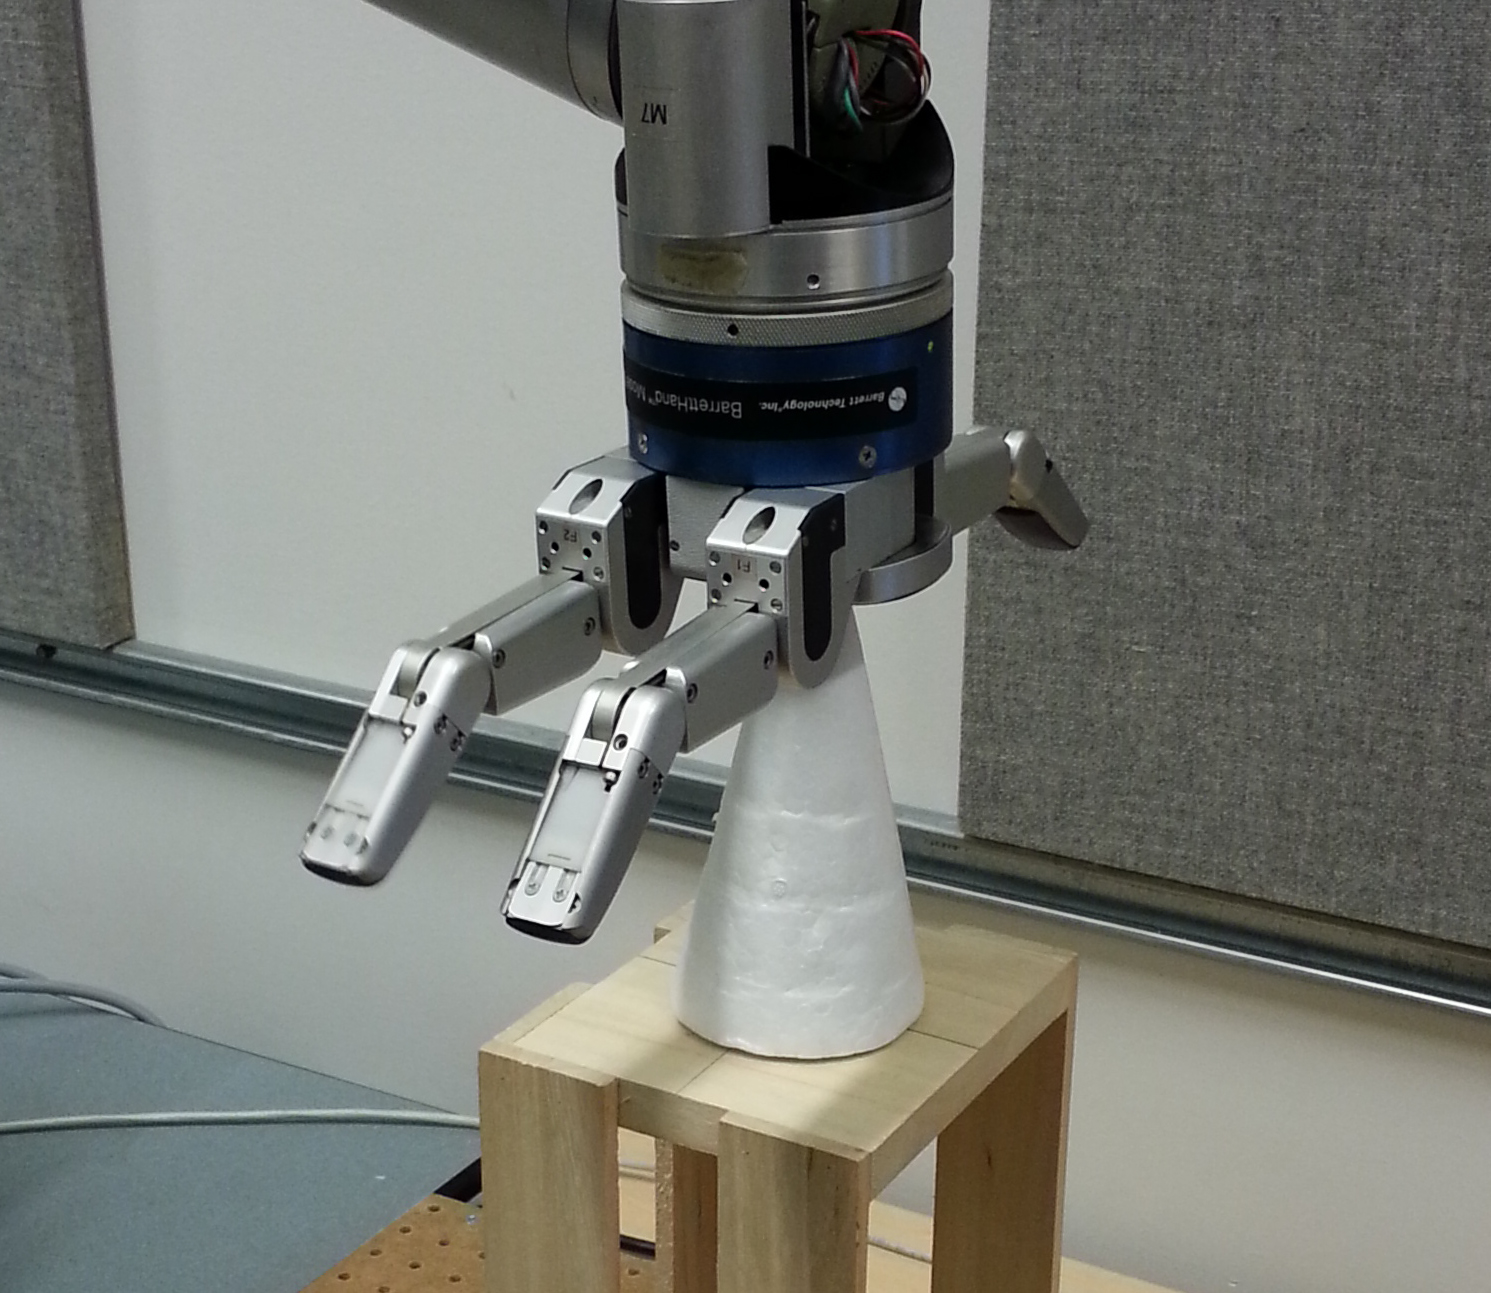
\includegraphics[width=0.75\textwidth]{updown.jpg}	
\end{figure}
\end{minipage}
\\[0.5cm]
\begin{minipage}{0.5\textwidth}
\qquad\quad \textbf{Top-down Tripod Precision} 
\begin{figure}[H]
	\centering
	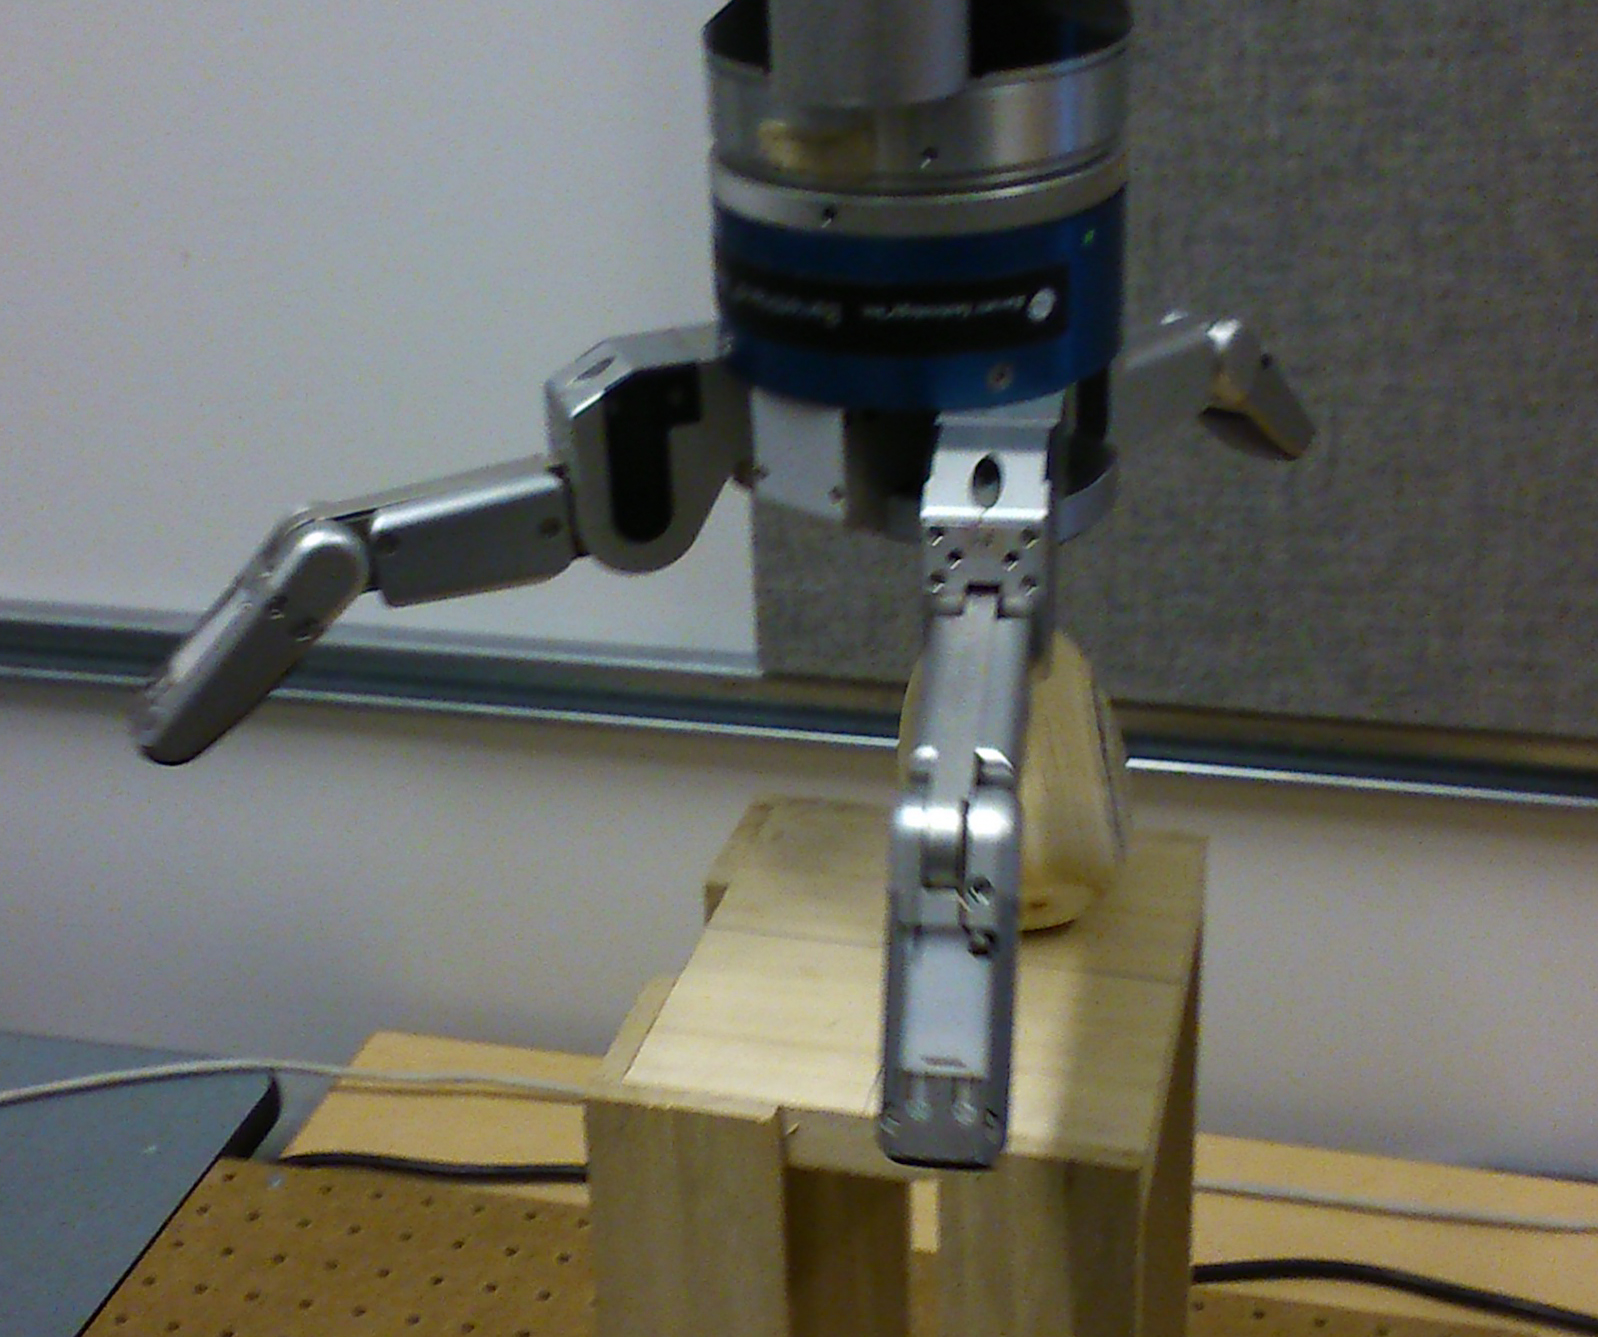
\includegraphics[width=0.75\textwidth]{tripod.jpg}	
\end{figure}
\end{minipage} 
\\[0.5cm]
\begin{minipage}{0.5\textwidth}
\qquad\quad \textbf{Side-on Heavy Wrap} 
\begin{figure}[H]
	\centering
	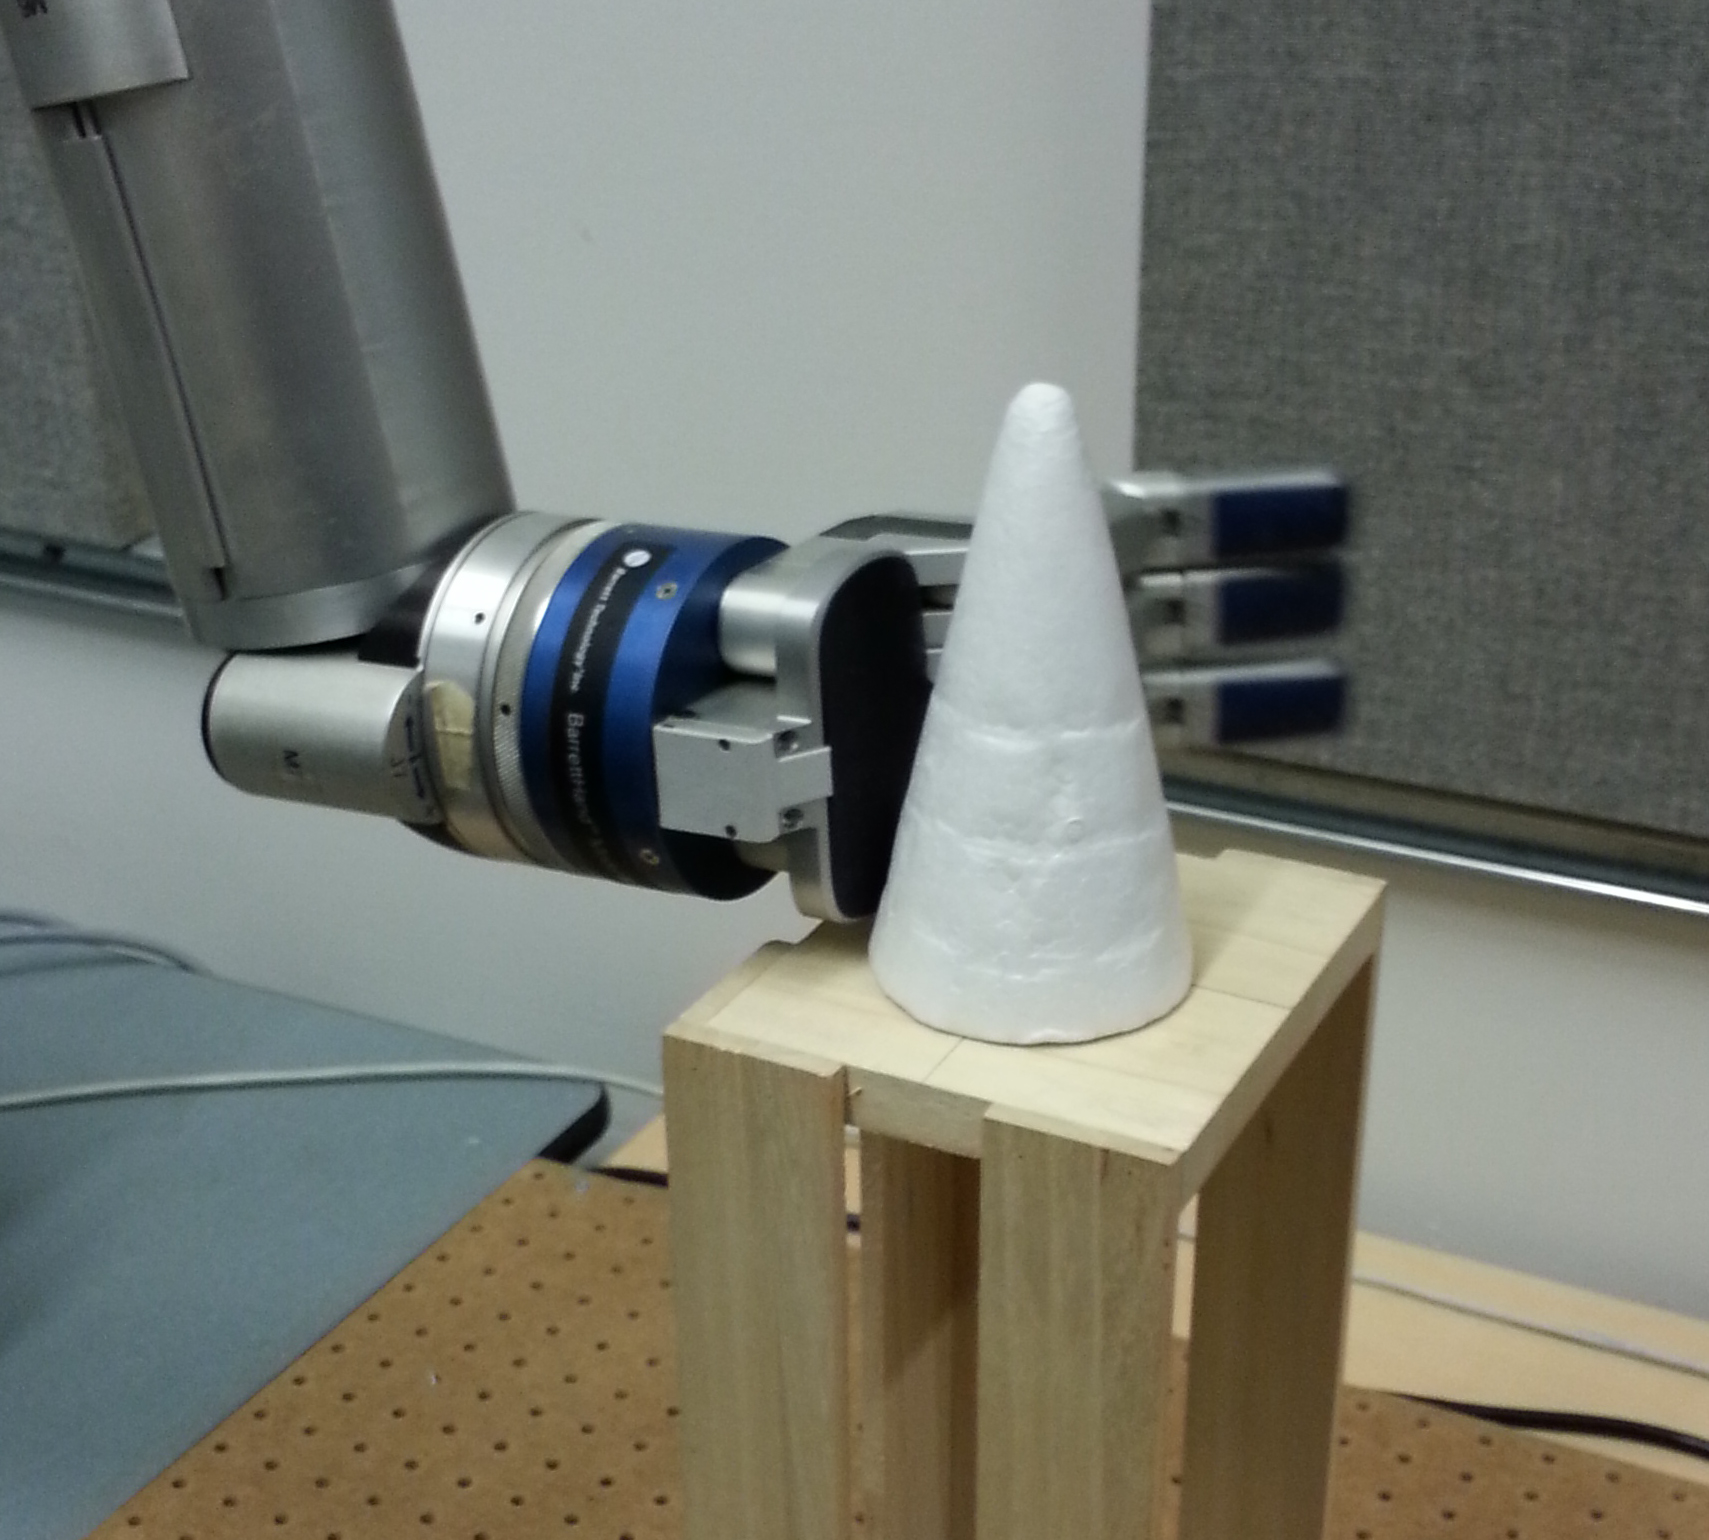
\includegraphics[width=0.8\textwidth]{heavywrap.jpg}	
\end{figure}
\end{minipage} 
\\[0.5cm]
\begin{minipage}{0.5\textwidth}
\qquad\quad \textbf{Side-on Power Grip} \quad as well as 

\qquad\quad \textbf{Side-on Prismatic Precision} 
\begin{figure}[H]
	\centering
	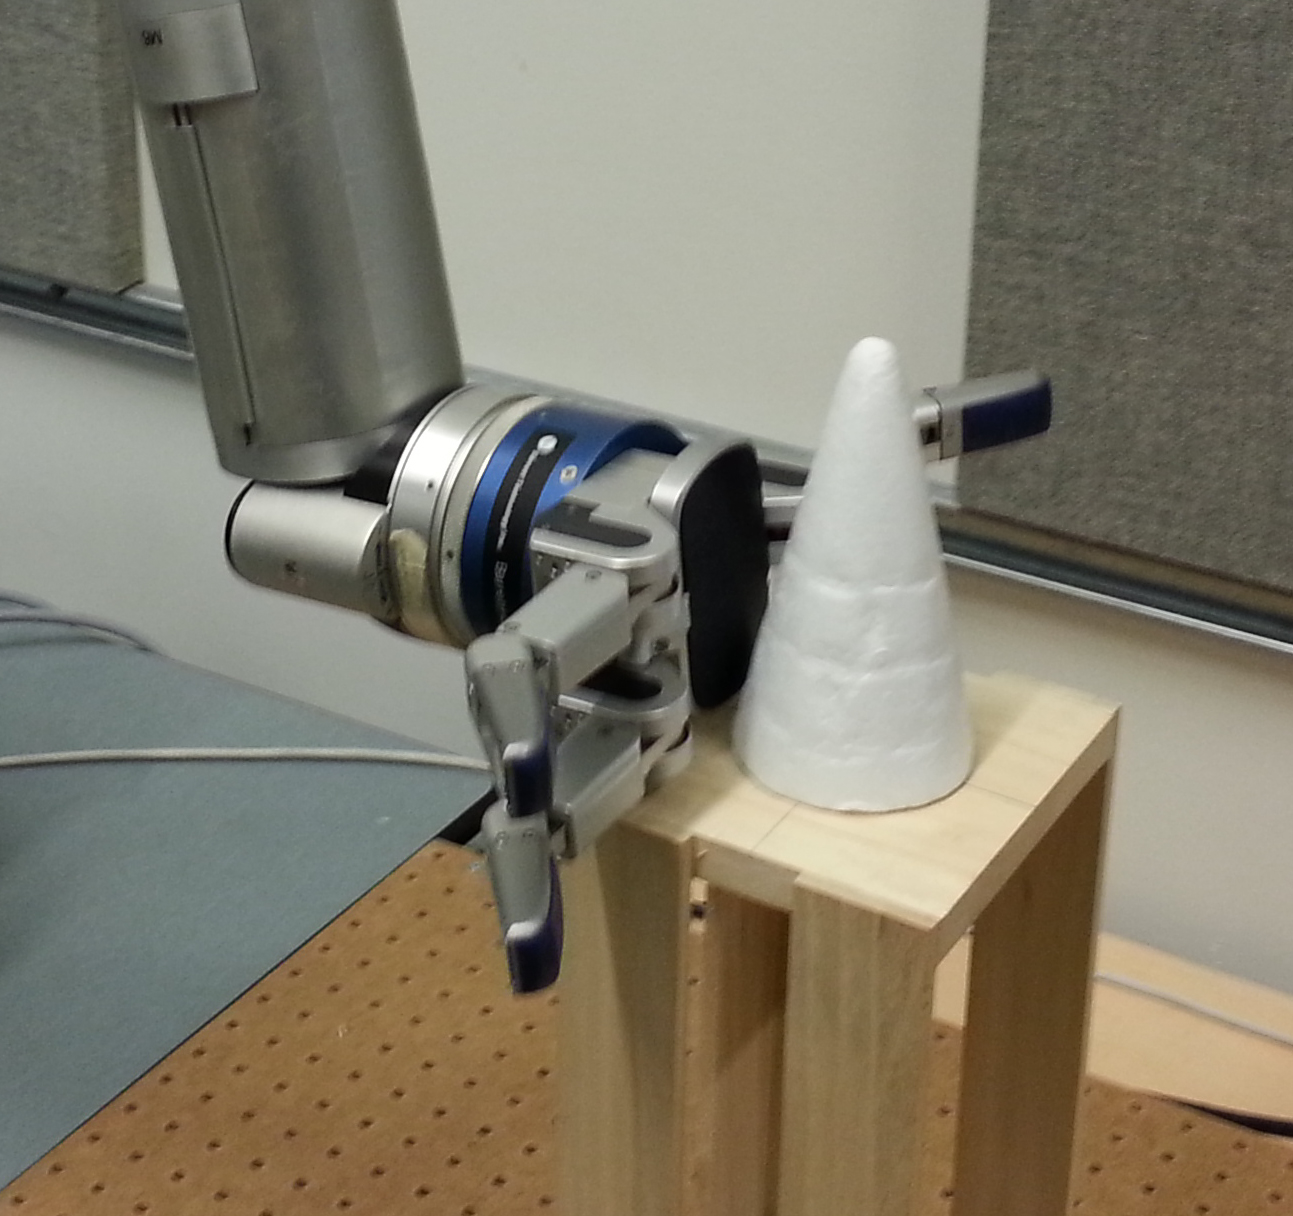
\includegraphics[width=0.85\textwidth]{powergrip.jpg}	
\end{figure}
\end{minipage}
\\[0.5cm]

Thus, each grasp is a combination of two factors: the position of the hand and the position of the fingers. The position of the hand, referred to as the "target position", can be either from the side (side-on) or from above (top-down). The position of fingers 1 and 2 can be at $0^\circ$ (prism), $30^\circ$ (tripod), or $180^\circ$ (wrap). When the user chooses one of the above grasps, the robot follows a fixed sequence of states:\\
\begin{description}
\item[First] Move to preparatory position.
\item[Second]  Prepare (preshape) the hand for the particular grasp type (prism, tripod, or wrap).
\item[Third]  Move to the target position (side-on or top-down).
\item[Fourth]  Close the hand on the object.
\item[Fifth]  Lift the object briefly and return it to the pedestal.
\item[Sixth]  Release the object and retreat to the preparatory position.
\end{description}

During steps 3-5, the following sensors are recorded and logged to disk:
\begin{itemize}
\item WAM joint positions
\item Finger joint positions (outer link)
\item Finger torques
\item 3D wrist forces
\item Palm and finger tactile pressures
\end{itemize}

The software is structured such that all menu options are executed asynchronously. The user always retains control and can cancel the current sequence at any time. Over time working with the robot we also found it necessary to add various facilities for identifying the name of the object currently being grasped, resetting the hand/WAM if they have controller issues, and recording a failed grasp. We use these annotations to sort and label our sensor data samples.

\subsection*{Data Collection}
The objects grasped varied in shape, size, symmetry, texture, weight, pliancy, and firmness. For details see Figure \ref{objects}. Each object was grasped several times with 3 (if possible) different grip strategies (Top-down Prismatic Precision, Heavy Wrap, and Power Grip). 

Data from many trials of grasping these objects were collected into log files. These files were then imported into \textsc{Matlab} and sorted by object and grasp type. From these files, we took only the interval during which the object was being grasped.

The finger joint positions were used to determine the time interval for sensor sampling. Initially, the finger torques were used for this purpose, but later in the project we encountered technical difficulties in communicating with the strain gages, and this method had to be altered. Luckily, the joint position data proved sufficient. As the two positional changes (i.e. the maximum and minimum of the derivative) mark start and end time point of each grasp, the specific time stamps for each trial could be calculated and used to find only the relevant data set for the neural network analysis. Subsequently, each object was assigned a label to run a classification.
\begin{figure}[t]
\begin{center}
	\hspace{-0.5cm}
	\includegraphics[width=0.45\textwidth]{objects.jpg}
	\caption{Set of grasped objects on which classification was performed. (1) styrofoam ball, (2) soft foam, (3) styrofoam cone, (4) foam square, (5) wood block, (6) plush octopus, (7) foam butterfly, (8) packaging tape, (9) rattan ball, (10) cookie cutter, (11) wooden egg, (12) football, (13) foam star, (14) drinking bottle, (15) cube, and (16) bean bag.}
	\label{objects}
\end{center}
\end{figure}

\subsection*{Neural Network}
To classify a grasp, the sensor data were normalized and used to train a three layer neural network. We read a total of 103 sensor values, and classified among 16 possible objects. Additionally, we formed a class \lq Failed Grasp\rq\ to which we assigned all failed grasps independent of the object, making for a total of 17 classes.

Therefore, the neural network consists of a 103 node input layer, a 25 node hidden layer, and a 17 node output layer. The implementation was largely based on the one found in Andrew Ng's Machine Learning course \cite{ML9}. Since this single hidden layer with 25 nodes was enough to perform robust character recognition in \cite{ML9}, it was deemed a satisfactory configuration for our purpose as well. Figure \ref{nn_config} depicts the nodes in the three layers of the neural network.

\newcommand{\vi}{\mathbf{v}_i}
\newcommand{\h}[1]{\mathbf{a}^{(#1)}}
\newcommand{\layer}[1]{\Theta^{(#1)}}
\newcommand{\e}{\mathbf{e}}
\newcommand{\sig}{\operatorname{sigmoid}}

After the first round of experiments, we used the labeled data we collected to train a separate neural network for each of the three chosen grasps. All 103 features were separately normalized before training. For each sensor $i$, the column vector $\vi$ of all samples becomes

$$ \vi = \frac{\vi - \operatorname{mean}(\vi)}{\operatorname{std}(\vi)} $$

Neural networks were trained using a cost function $J(\Theta)$ similar to $K$ regularized logistic regressions, where $K$ is the number of classes, 17. We also added a regularization term with an adjustible weight $\lambda$. The training algorithm iteratively finds the parameters $\Theta$ which minimize the cost function $J(\Theta)$ by computing the cost function gradient $\frac{\partial J(\Theta)}{\partial\Theta}$ in the neural network at each step over all training examples. For full details of the algorithm, see \cite{ML9}.

We produced a variety of different networks with different regularization weights from $\lambda = 1$ to $\lambda = 1000$. 20\% of the collected time points from each grasp were set aside as a test set to verify our results.\\
\begin{figure}[t]
\begin{center}
	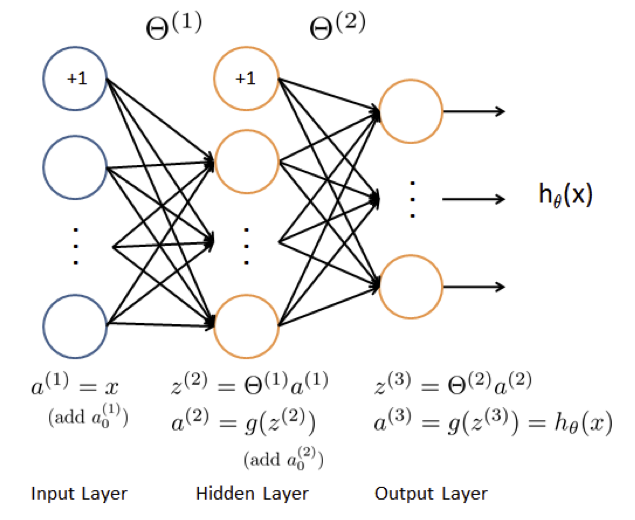
\includegraphics[width=.45\textwidth]{nn.png}
	\caption{A three layer neural network for the classification of grasped objects from finger pose, wrist force, and tactile pressure data. Taken from Programming Exercise 4 in \cite{ML}.}
	\label{nn_config}
\end{center}
\end{figure}
\vspace{-0.5cm}

\quad At this point a module was added to the software which predicted the object being grasped, given one or more samples of the above sensor data. The final version of the software printed out the name of the object which it ``sensed'', while lifting the object from the pedestal. This was implemented by taking a single time slice of sensor data while grasping an object, and feeding it forward through each layer of the neural network. In each layer,

$$ \h{i+1} = \sig\bigl(\bigl[\e~~\h{i}\bigr] \layer{i}\bigr) $$
\begin{eqnarray*}
 \text{where } &&\h{1} \in \mathbb{R}^{m\,\mathrm{x}\,103} = \text{the sensor samples} \\
 				&&\h{i} = \text{output of layer } i \\
 				&&\layer{i} = \text{parameters of layer } i \\
				&&\e = \text{column of all ones} \\
				&&\sig(z) = \frac{1}{1 + \mathrm{e}^{-z}}
\end{eqnarray*}

The final prediction is taken as the label which was assigned the maximum probability by the output layer:

$$ \operatorname{object} = \text{index of } \max(\h{3}) $$
